\documentclass[notitlepage]{article}
\usepackage[utf8]{inputenc} 
\usepackage{geometry} 		
\usepackage{chngcntr}
\usepackage{amsmath} 			
\usepackage{amssymb}			
\usepackage{mathtools}		
\usepackage{comment} 			
\usepackage{mdframed}			
\usepackage{xcolor}				
\usepackage{fancyhdr}			
\usepackage{listings}			
\usepackage{color}				
\usepackage{tikz}	
\usepackage{tasks}			
\usepackage{exsheets}	
\usepackage{blindtext}	
\usepackage{array}			
\usepackage{empheq}
\usepackage{caption}
\usepackage{pdfpages}
\usepackage{tabularx}
\usepackage{lscape}

\geometry{ 						%Format titlepage (interrupted by newgeometry)
	a4paper,
	total={170mm,257mm}%,
	%left=0mm,
	%top=0mm,
}

%START DEFINE YOUR VARIABLES HERE

\newcommand{\documentName}{Software Design Specification}
\newcommand{\projectName}{Label Refinement by Behavioral Similarity}

%END DEFINE YOUR VARIABLES HERE

\title{%
	\documentName\text{ } \\
  \large \projectName\text{ } \\
  }

\author{
	\large \underline{Document owners:}\\ 
	Bianka Bakullari\\
	\texttt{}
	Christopher Beine\\
	\texttt{}
	Nicole Ventsch\\
	\texttt{}
	Juan Garza\\
	\texttt{}
}

\date{\small{Last edited: \today}}

\pagestyle{fancy}
\fancyhf{}
\rhead{}
\lhead{\documentName\space-\space\projectName}

\makeatletter					%Prefix to add ToC to titlepage
\newcommand*{\toccontents}{\@starttoc{toc}}
\renewcommand*\contentsname{}
\makeatother
                  

\begin{document}

\begin{titlepage}
\clearpage\maketitle			%Clear title page
\thispagestyle{fancy}
\tableofcontents
\end{titlepage}

\rfoot{\thepage}				%Start printing page-numbers, after title page.

\newgeometry{ 					%Default page formatting on-going #1
	total={170mm,257mm},
	left=20mm,
	top=25mm,
    bottom=30mm					%Causes warning
}

\begin{flushleft}				%Default page formatting on-going #2


\section{Introduction}
\subsection{System Overview}
\subsection{Design Map}
\subsection{Supporting Materials}
\subsection{Definitions and Acronyms}

\section{Design Considerations}
\subsection{Assumptions and Dependencies}
\subsection{General Constraints}
\subsection{Goals and Guidelines}
\subsection{Development Methods}

\section{Architectural Strategies}
{\color{gray} **** under construction ****}
\begin{itemize}
	\item Factory Pattern
	\item Decorator (Variaton)
\end{itemize}

{\color{gray} ***************************}
\section{System Architecture}
\includegraphics[scale=0.4]{"UML_Architecture/Architecture Overview".png}

\subsection{Client Machine}
\subsection{Front-end}
\subsection{Refining Label API}
\subsection{File Store}
\subsection{Refining Event Labels}
\begin{landscape}
\subsection{Event Log Converter}
\includegraphics[width=\columnwidth]{"UML_Architecture/Event Log Converter CD".png}
\end{landscape}
\section{Policies and Tactics}

\section{Detailed System Design}
The main algorithm "Refining Event Labels" will be split up into multiple modules that contain the main parts of the algorithm. These modules will be explained in detail in the following subsections.
\subsection{Module 1.1: File Converter}
\textit{Name}: File Creator

\textit{Type}: module

\textit{Description}: This module is responsible for creating a table from the data the user uploads. The event log provided by the user is read and stored internally containing all the original columns. 

\textit{Attributes}: None

\textit{Resources}: None

\textit{Operations}: 
\medskip

\par
\begingroup
\leftskip4em
\textbf{1.1.1}

\textit{Name}: get\_event\_log\_from\_file()

\textit{Arguments}: path to a log file in csv format or XES format

\textit{Returns}: event log in XES format

\textit{Description}: The file at the path the user enters is read and stored in XES format. In case the file is originally in csv format, the file is first converted to XES format and then stored.

\textit{Precondition}: the path provided by the user leads to a csv file or an XES file

\textit{Postcondition}: the table is stored internally as an XES file

\textit{Exceptions}: None
\par
\endgroup

\medskip

\par
\begingroup
\leftskip4em
\textbf{1.1.2}

\textit{Name}: read\_XES()

\textit{Arguments}: file in XES format

\textit{Returns}: event log 

\textit{Description}: The XES file is read and stored as a table containing the original columns.

\textit{Precondition}: an XES file was created using get\_event\_log\_from\_file()

\textit{Postcondition}: a table containing all original columns is stored internally 

\textit{Exceptions}: None
\par
\endgroup

\medskip

\subsection{Module 1.2: Preprocessing Log}
\textit{Name}: Preprocessing Log

\textit{Type}: module

\textit{Description}: This module is responsible for preprocessing the data. It is checked if the table provided by the user contains the right variables and an error is produced if is does not have. Moreover, a table containing all unique traces and the list of IDs corresponding to these traces is created.

\textit{Attributes}: None

\textit{Resources}: None

\textit{Operations: }
\medskip


\par
\begingroup
\leftskip4em
\textbf{1.2.1} 

\textit{Name}: check\_event\_log()

\textit{Arguments}: table imported using read\_XES() 

\textit{Returns}: Boolean (True or False)

\textit{Description}: It is checked whether the table is actually an event log, i.e., whether it contains an activity column, an ID column and a time stamp column. If these exist in the table, "True" will be returned, otherwise "False" will be returned. 

\textit{Precondition}: a file was created using read\_XES()

\textit{Postcondition}: if "True" is returned, the file is actually an event log, otherwise the file does not contain the necessary variables and an error will be displayed

\textit{Exceptions}: None
\par
\endgroup

\medskip

\par
\begingroup
\leftskip4em
\textbf{1.2.2}

\textit{Name}: lookup\_table()

\textit{Arguments}: table with all original columns

\textit{Returns}: lookup table containing a "variants" column and an "ID" column

\textit{Description}: The table is converted, so that we get a table containing the unique variants for the IDs ordered by their time stamp and the set of IDs corresponding to the variant. In this lookup table, the variants are stored as arrays and the corresponding IDs as a list.

\textit{Precondition}: the provided file is an event log

\textit{Postcondition}: a lookup table is stored containing the variants and IDs corresponding to those variants

\textit{Exceptions}: None

\par
\endgroup

\medskip

\par
\begingroup
\leftskip4em
\textbf{1.2.3}

\textit{Name}: get\_variants()

\textit{Arguments}: look-up table with variants and IDs for each variant

\textit{Returns}: set of unique trace variants

\textit{Description}: We create a set containing all the variants so that we can approach them when calculating the mappings later. Here we do not need to have access to the IDs.

\textit{Precondition}: The first column of the look-up table contains all trace variants

\textit{Postcondition}: a non-empty set containing the arrays describing each variant

\textit{Exceptions}: None

\par
\endgroup

\subsection{Module 2: Customize}
\textit{Name}: Customize

\textit{Type}: module

\textcolor{red}{Operations: setCandidates, getCandidates, setThresholds, getThresholds}




\subsection{Module 3: Download}
\textit{Name}: File Creator

\textit{Type}: module

\textcolor{red}{Operations: setCandidates, getCandidates, setThresholds, getThresholds}

\subsection{Module 4: Calculate costs}
\textit{Name}: Cost function

\textit{Type}: module

\textit{Description}: This module is responsible for calculating the costs of all mappings between each pair of variants and selecting the optimal mapping with the least costs. 

\textit{Attributes}: None

\textit{Resources}: The weights used for the calculation of costs

\textit{Operations}: 
\medskip

\par
\begingroup
\leftskip4em
\textbf{4.1} 

\textit{Name}: mappings()

\textit{Arguments}: two distinct trace variants 

\textit{Returns}: a set of possible mappings

\textit{Description}: For each pair of variants we obtain the set of common activity labels occurring in both variants. If this set is empty, no mapping is possible. Otherwise, if none of the common labels appears more than once in any of the variants, the unique mapping is yielded. In the other case, all combinations of possible mappings are yielded as a set where each mapping is an array of pairs of the positions that were matched together.

\textit{Precondition}: We go through all pairs of trace variants yielded by get\_variants()

\textit{Postcondition}: For each mapping, the cost function is computed

\textit{Exceptions}: None
\par
\endgroup


\medskip

\par
\begingroup
\leftskip4em
\textbf{4.2} 

\textit{Name}: cost\_mapping()

\textit{Arguments}: two trace variants and a mapping between them

\textit{Returns}: the cost of the mapping as a real number

\textit{Description}: For each pair in the mapping we count the number of distinct predecessors and successors and the distances to other matched pairs. We sum over these costs for all matched pairs and also add the number of unmatched labels appearing in the traces. Each summand is weighted with a corresponding weight.
Simultaneously we save all costs between pairs of variants in a list so that we can pick the minimal one.

\textit{Precondition}: We calculate the costs for each mapping yielded by mappings().

\textit{Postcondition}: For each mapping, the corresponding cost is computed.

\textit{Exceptions}: None
\par
\endgroup


\medskip

\par
\begingroup
\leftskip4em
\textbf{4.3} 

\textit{Name}: cost\_matrix()

\textit{Arguments}: the cost of the optimal mapping for each pair of variants

\textit{Returns}: a symmetrical 2-dimensional matrix

\textit{Description}: The matrix contains 0s in the diagonal and the entry in position $[i][j]$ corresponds to the cost of the optimal mapping between variant $i$ and variant $j$. 

\textit{Precondition}: We can obtain the cost of the optimal mapping between two variants by choosing the minimal entry in the list of costs of their possible mappings saved in cost\_mapping().

\textit{Postcondition}: For each pair of variants, the cost of the optimal mapping is known.

\textit{Exceptions}: None
\par
\endgroup


\medskip

\par
\begingroup
\leftskip4em
\textbf{4.4} 

\textit{Name}: graph()

\textit{Arguments}: the cost of the optimal mapping for each pair of variants and the set of variants

\textit{Returns}: a connected graph

\textit{Description}: For each variant there is a set of vertices corresponding to the events occuring in the variant. Each edge only connects matched pairs and for the pairs being in the candidate set the weight of each edge corresponds to the cost of the optimal mapping. Otherwise the weight of the edge is 0.

\textit{Precondition}: The weights for the edges are obtained from the cost\_matrix().

\textit{Postcondition}: Each variants has to be identifiable in the graph in order to be able to do the horizontal and vertical refinements in the next steps.

\textit{Exceptions}: None
\par
\endgroup


\subsection{Module 5: Horizontal clustering of variants}
\textit{Name}: Label refinement based on clusters

\textit{Type}: module

\textcolor{red}{Operations: clusterdetectionrelation, refinement}

\subsection{Module 6: Vertical Refinement}
\textit{Name}: Label refinement within variant

\textit{Type}: module

\textcolor{red}{Operations: relabel(graph, cluster, threshold)}



\subsection{Module 7: Post-Processing}
\textit{Name}: Embed refinements into original log 

\textit{Type}: module

\textcolor{red}{Operations: refinedlog(graph, lookup table)}










\section{User Interface Design}
\subsection{Application Control}

In the project, we will implement a web service. The web client will have a rather plain design that should focus on the main activities the service should provide, which are uploading event logs in csv or XES format, setting the threshold for the label refinement algorithm and download the refined log after the algorithm is finished. There will be buttons used to upload the file, apply the algorithm and download the refined event log. Moreover, the screens will have short explanations telling the user what to do (if not self-explanatory). For setting the thresholds, two boxes will be provided that include the default thresholds, but new values can be entered by the user. A draft of each of the main screen can be found in the next section, section 6.2.

\subsection{The Screens}

The main screens will be visualized in the following subsections. In these screens include the main functionalities, which are described in the former section. The following diagram will show the flow of control through the screens.  

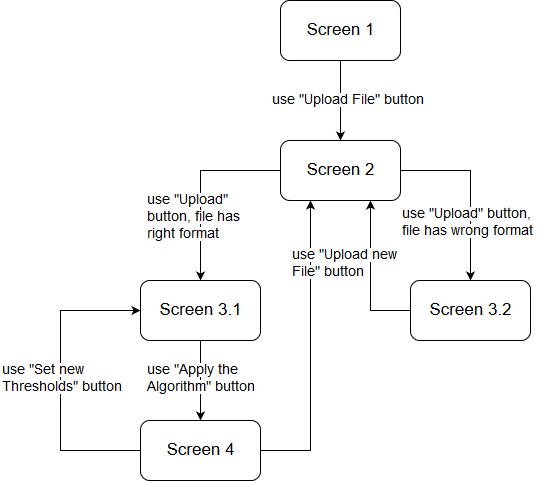
\includegraphics[scale=0.7]{ScreenFlow.png}

\subsubsection{Screen 1}

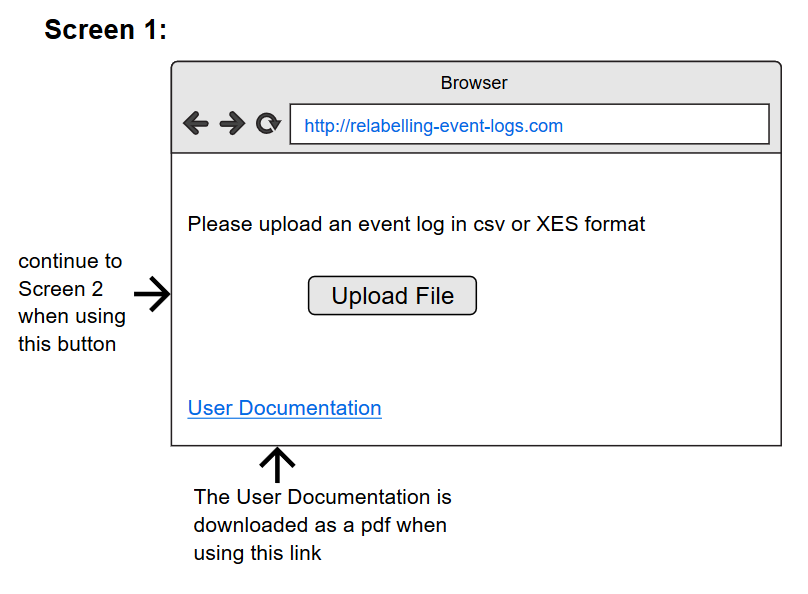
\includegraphics[scale=0.8]{InterfaceMockup1.png}


The first screen visible to the user will show a description saying that an event log in csv of XES format should be uploaded. Moreover, a button "Upload File" is visible. By using this button, the user will continue to Screen 2. At the end of the page, there will be a link called "User Documentation". By clicking on this link, the User Documentation will be downloaded in pdf format.
\subsubsection{Screen 2}

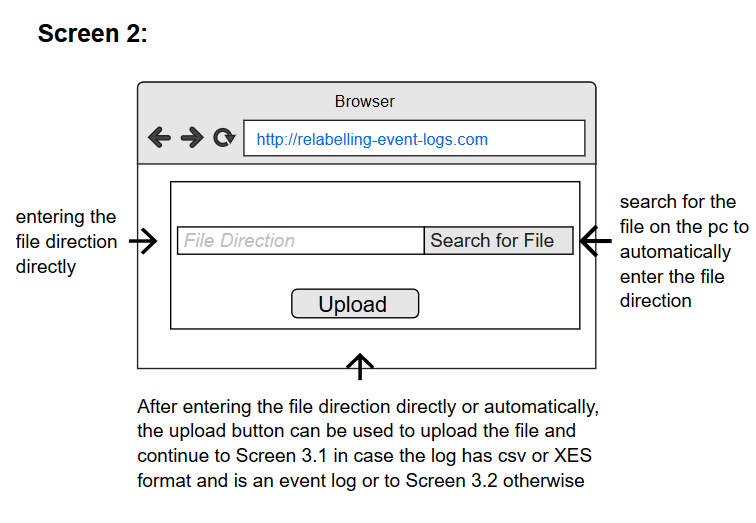
\includegraphics[scale=0.9]{InterfaceMockup2.png}

In the second screen visible to the user, the user can enter the file direction of the event log he wants to upload. He can either directly type in the direction into the "File Direction" field or use the "search for File" button to search for a file on his pc, so that the direction will automatically be filled in after selecting a file.

After using one of this alternatives, he can use the "Upload" button to upload the file with the given directory. In case this file is an event log, i.e., the data contains at least the attributes "id", "time stamp" and "activity name", and has either csv or XES format, the user will continue to Screen 3.1. If one of these conditions is not satisfied, he will continue to Screen 3.2. 


\subsubsection{Screen 3.1}
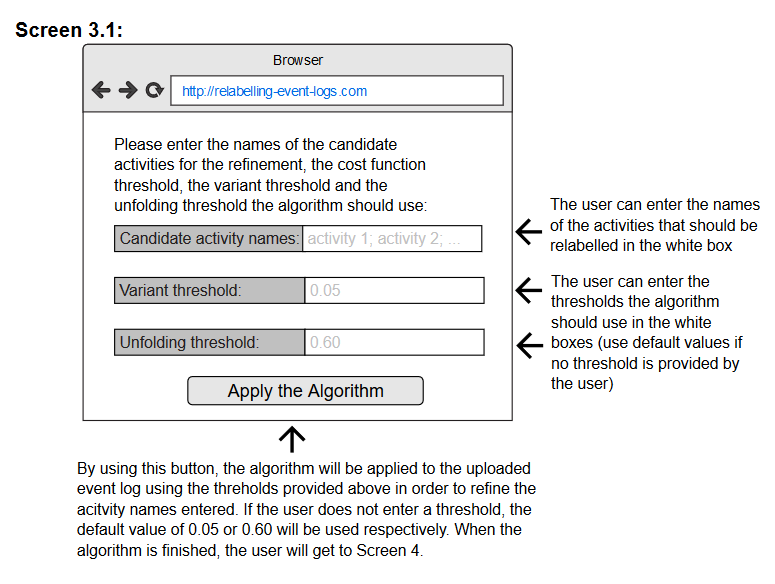
\includegraphics[scale=0.9]{InterfaceMockup3-1.png}

This screen appears if the file uploaded by the user meets the requirements. In this screen, the user can set the thresholds for the algorithm, i.e., the variant and the unfolding threshold. He can enter these in the corresponding white boxes. If he does not enter the thresholds, the default values of 0.05 and 0.60 will be used respectively. Using the button "Apply the Algorithm", the web service will start applying the algorithm using the provided thresholds. After the algorithm is finished, the user will get to Screen 4.

\subsubsection{Screen 3.2}
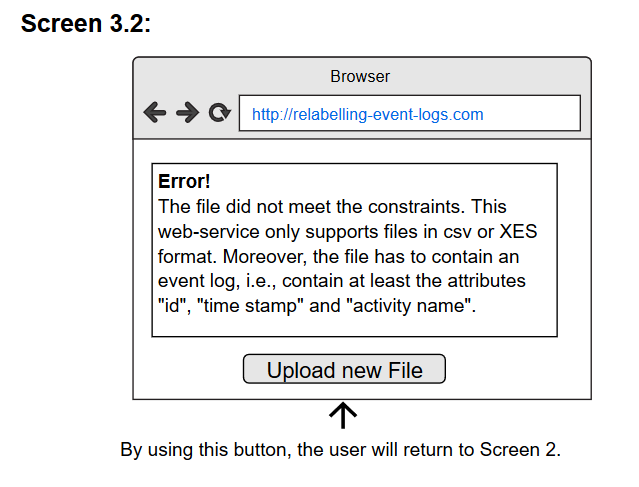
\includegraphics[scale=0.9]{InterfaceMockup3-2.png}

This screen appears if the upload was not successful because the file did not meet the assumptions. If the file does not have the right format, the user can click on the button "Upload new File" to return to Screen 2 and upload a file that meets the constraints.


\subsubsection{Screen 4}
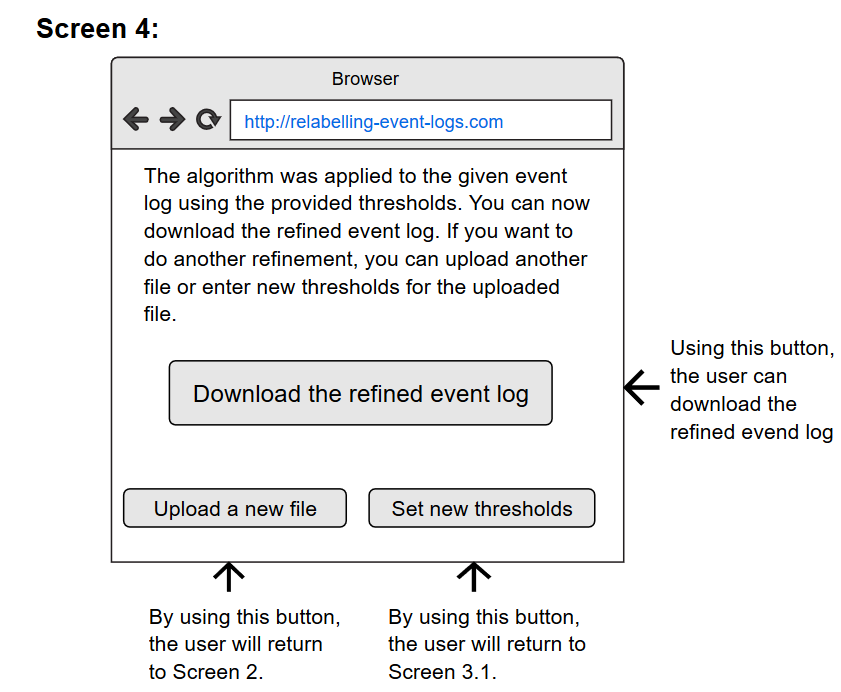
\includegraphics[scale=0.8]{InterfaceMockup4.png}

This Screen will be shown after finishing the algorithm. The user can now download the refined log using the corresponding button. After this step, the user is done and can exit the page, but if he also wants to apply the algorithm to another event log or to the same event log using different thresholds, he can use the corresponding buttons and will be redirected to Screen 2 or Screen 3.1 respectively.


%\newpage
%\bibliographystyle{plain}
%\bibliography{references}  




%\addcontentsline{toc}{chapter}{\textbf{References}}
\end{flushleft}
%\bibliography{uw-ethesis}
% Tip 5: You can create multiple .bib files to organize your references. 
% Just list them all in the \bibliogaphy command, separated by commas (no spaces).

% The following statement causes the specified references to be added to the bibliography% even if they were not 
% cited in the text. The asterisk is a wildcard that causes all entries in the bibliographic database to be included (optional).


\begin{thebibliography}{5}
\bibitem{paper}
Lu, Xixi, et al. "Handling duplicated tasks in process discovery by refining event labels." International Conference on Business Process Management. Springer, Cham, 2016.

\bibitem{matchings}
Xixi Lu1, Dirk Fahland, Frank J.H.M. van den Biggelaar, Wil M.P. van der Aalst. "Detecting Deviating Behaviors without Models."


\end{thebibliography}










\end{document}
